\subsubsection{User Interfaces}

            This section describes the components of the user interface. The components are grouped into views which allow the user to interact with a particular state or feature of the application. Some views may extend beyond the edges of the smart phone's screen size, in that case the figure will attempt to show multiple versions of a view. The figures shown do not represent every possible combination of states the application may have.

            \paragraph{UI-1: Home Screen}

            The Home Screen is the view that will appear to the user when the MDApp is first started. It will act as a jump off point to guide the user through the app, showing quick links with a short description. When the MDApp is started for the first time, there will be no data or images available to view in the Analysis or Archive views. The MDApp will therefore not display the quick link for the Analysis View or the Archive View, only the Camera View.

                \begin{figure}[H]
                    \centering
                    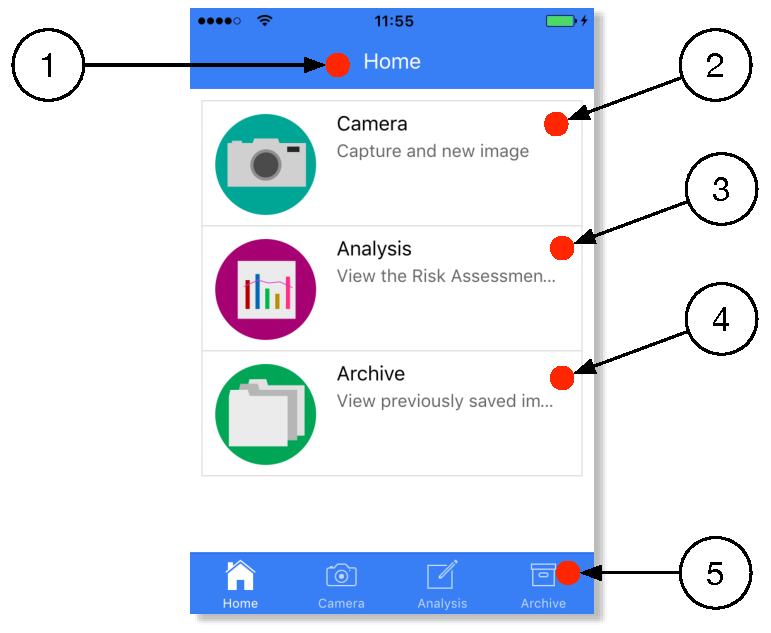
\includegraphics[height=7cm]{assets/GUI/HOME_01.pdf}
                    \caption{UI-1: Home Screen}
                    \label{fig:ui-1}
                \end{figure}

                \begin{itemize}
                    \item[1] View Title, every view shall have a title.
                    \item[2] Quick link to the Camera View.
                    \item[3] Quick link to the Analysis View, only visible if an image has already been captured.
                    \item[4] Quick link to the Archive View, only visible if images have been saved to the archive.
                    \item[5] Tab-bar navigation element. This component is always visible, in all of the app’s views.
                \end{itemize}

            \paragraph{UI-2: Camera View}

            The Camera View will automatically start the real time camera preview, displaying an image of what the camera is currently pointing at. Some visual indicators will help the user to center the skin lesion in the image. Because the user might be taking an image of her or his own body it might be difficult to click a button while holding the camera steady. Therefore touching anywhere on the camera preview area will trigger an image capture. An audible “shutter” noise will also signal the user that an image has been captured.

                \begin{figure}[H]
                    \centering
                    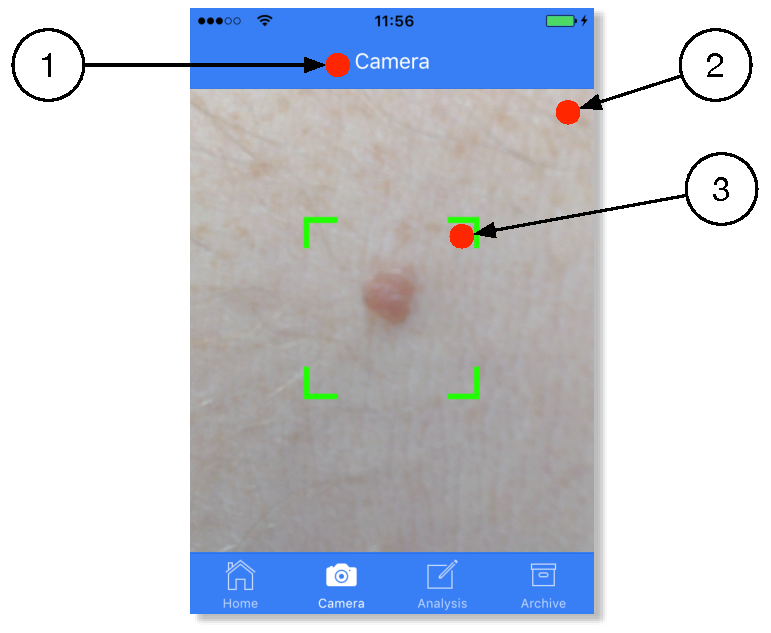
\includegraphics[height=7cm]{assets/GUI/CAMERA_01.pdf}
                    \caption{UI-2: Camera View}
                    \label{fig:ui-2}
                \end{figure}

                \begin{itemize}
                    \item[1] View Title, every view will have a title.
                    \item[2] Realtime camera preview.
                    \item[3] Crosshairs, visual markers that indicate where the center of the image is. The user should attempt to keep the lesion within the markers, but filling the marked area as much as possible. (limited by the focal range of the smart phone’s camera)

                \end{itemize}

            \paragraph{UI-3: Analysis View}

            The Analysis View presents the current state of processing and the results of any finished calculations. When the border calculation is finished, the Smartphone User is promoted to confirm that the border was precisely calculated. If not the app will return the Smartphone User to the Camera View to capture another version of the image. The risk assessment data will be presented to the Smartphone User below the border image along with a summary and recommendation as text ( not shown in figure ref[] ). The Smartphone User can also add addition text as metadata and specify where on her/his body the skin lesion was located. The Smartphone User also has the option to save the image and data to the archive.

                \begin{figure}[H]
                    \centering
                    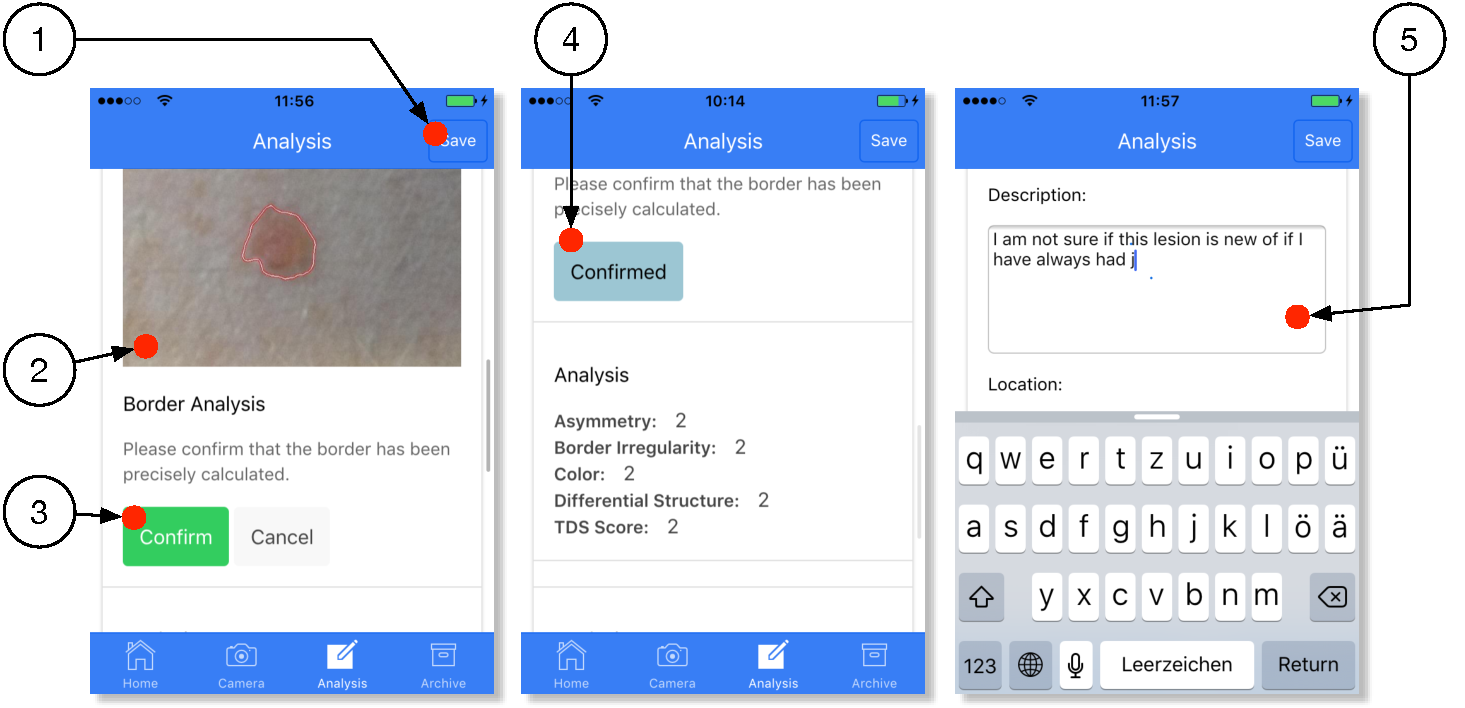
\includegraphics[height=7cm]{assets/GUI/ANALYSIS.pdf}
                    \caption{UI-3: Analysis View}
                    \label{fig:ui-3}
                \end{figure}

                \begin{itemize}
                    \item[1] Save button.
                    \item[2] Border Analysis preview
                    \item[3] Confirm and Cancel buttons with which the Smartphone User may confirm or reject that the border has been precisely calculated.

                    \item[4] Once confirmed, the button becomes an indicator that the border was confirmed. It is no longer clickable in this state.

                    \item[5] Additional metadata may be entered by the Smartphone User as text. Upon clicking a text input field the smartphone’s native text entry keyboard element will appear.

                \end{itemize}

            \paragraph{UI-4: Archive List View}

                \begin{figure}[H]
                    \centering
                    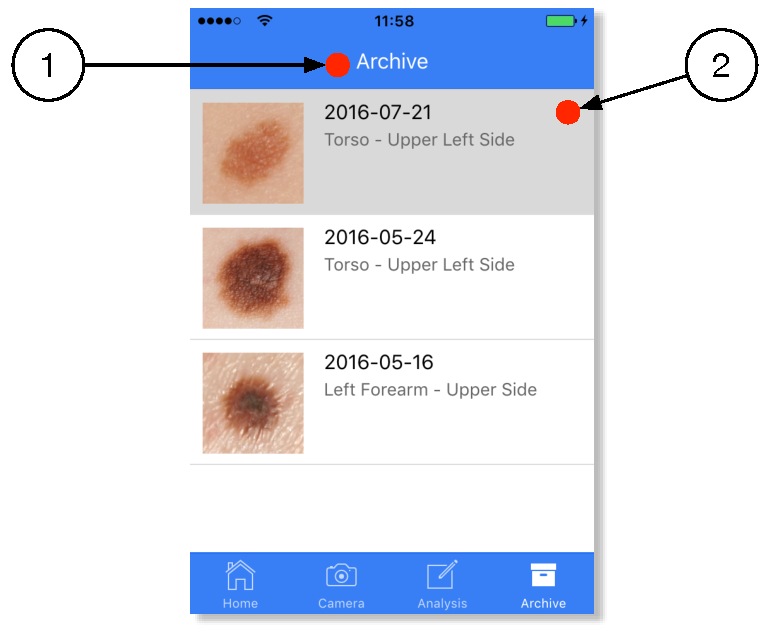
\includegraphics[height=7cm]{assets/GUI/ARCHIVE_01.pdf}
                    \caption{UI-4: Archive List View}
                    \label{fig:ui-4}
                \end{figure}

            \paragraph{UI-5: Archive Detail View}

                \begin{figure}[H]
                    \centering
                    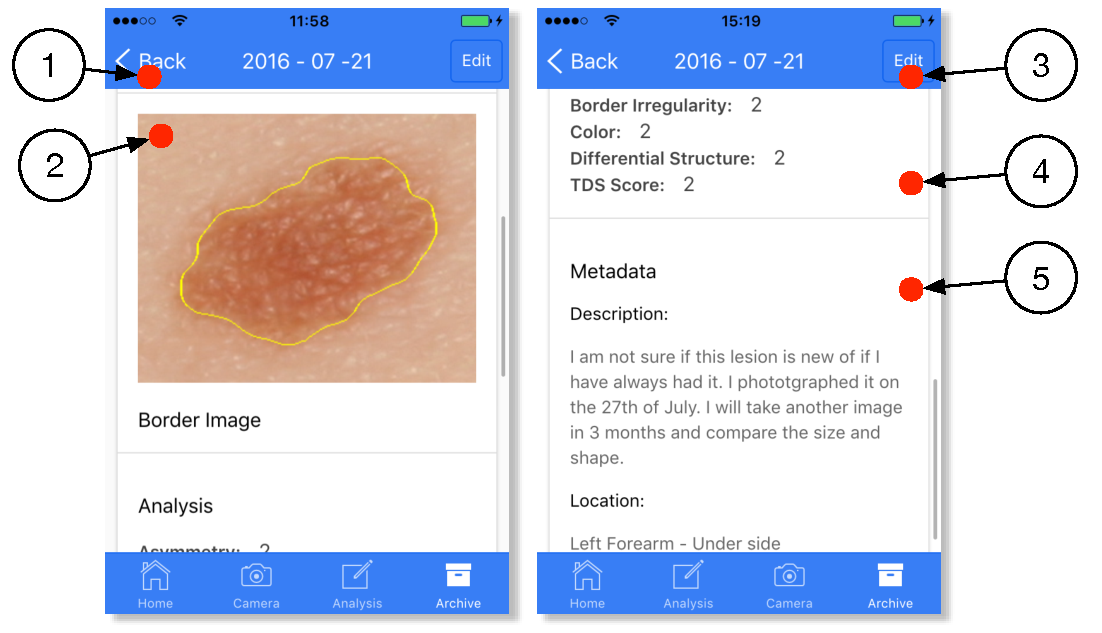
\includegraphics[height=7cm]{assets/GUI/ARCHIVE_02.pdf}
                    \caption{UI-5: Archive Detail View}
                    \label{fig:ui-5}
                \end{figure}


        \subsubsection{Software Interfaces}

            \paragraph{SI-1 : Smartphone Camera }
                The MDApp will interface with the Smartphone's camera hardware via the systems camera API.

                \begin{itemize}[leftmargin=1.4cm]
                    \item[SI-1.1 : ] The MDApp shall activate the camera when needed and be able to receive a live preview stream from the camera.
                    \item[SI-1.2 : ] If the native API allows, the MDApp should set to camera’s focus mode to Macro.
                    \item[SI-1.3 : ] If the native API allows, the MDApp should register a call back to be informed when the camera’s autoFocus has focused.
                    \item[SI-1.4 : ] The MDApp shall signal the camera to capture the highest resolution image possible when the Smartphone User triggers an image capture event.

                \end{itemize}

            \paragraph{SI-2 : Smartphone File System }
                Captured images and Border Analysis images must be stored on the Smartphone File System in such a manner so that they are accessible by the Smartphone User in the native methods. The native file access, file handling, and backup methods for the respective Smartphone platform shall apply to files created and captured by the MDApp

        \subsubsection{Communication Interfaces}

            \paragraph{CI-1 : Border Extraction Service }

                The Border Extraction Service is an online web based service that the MDApp can communicate with for the purpose of extracting the precise border information from a captured image of a skin lesion.

                \begin{itemize}[leftmargin=1.4cm]
                    \item[CI-1.1 : ] The MDApp will upload a captured skin lesion image to a web-based Border Extraction Service. The method for uploaded as part of a multipart/form-data html POST method.
                    \item[CI-1.2 : ] The MDApp will receive a confirmation from the service as JSON, including an id that will be used to poll the service for progress.
                    \item[CI-1.3 : ] The MDApp will poll the online service regularly, the service will indicated that the Border Extraction processes is in progress or has finished, in which case it will also include the url where the border image can be downloaded.
                    \item[CI-1.4 : ] The MDApp will download the border data image from the Border Extraction Service

                \end{itemize}

            \paragraph{CI-2 : Risk Assessment Service }

                The Risk Assessment Service is an online web based service that the MDApp can communicate with for the purpose of evaluating the risk of a skin lesion being a melanoma.

                \begin{itemize}[leftmargin=1.4cm]
                    \item[CI-2.1 : ] The MDApp will upload a captured skin lesion image to a web-based Border Extraction Service. The method for uploaded as part of a multipart/form-data html POST method.

                \end{itemize}